%************************************************
\chapter{Appendix}\label{ch:appendix}
%************************************************
\begin{table}[ht]
    \myfloatalign
    \begin{tabularx}{\textwidth}{rrr} \toprule
        \tableheadline{Mels} & \tableheadline{Hz}
        & \tableheadline{Filterbank} \\ \midrule
        % Phantoms take care of right-alignment (works iff monospaced digits)
        0    & 0\phantom{.0} & 0 \\
        105  & 68.5   & 2 \\
	        210  & 143.7  & 4 \\
	        315  & 226.2  & 7 \\
        420  & 316.8  & 10 \\
        525  & 416.3  & 13 \\
        630  & 525.5  & 16 \\
        735  & 645.4  & 20 \\
        840  & 777\phantom{.0} & 24 \\
        945  & 921.5  & 29 \\
        1050 & 1080.1 & 34 \\
        1155 & 1254.4 & 40 \\
        1260 & 1445.4 & 46 \\
        1365 & 1655.3 & 53 \\
        1470 & 1885.7 & 60 \\
        1575 & 2138.6 & 68 \\
        1680 & 2416.3 & 77 \\
        1785 & 2721.2 & 87 \\
        1890 & 3055.9 & 97 \\
        1995 & 3423.3 & 109 \\
        2100 & 3826.7 & 122 \\
        2205 & 4269.5 & 136 \\
        2310 & 4755.7 & 152 \\
        2415 & 5289.4 & 169 \\
        2520 & 5875.3 & 188 \\
        2625 & 6518.6 & 209 \\
        2730 & 7224.8 & 231 \\
        2835 & 8000\phantom{.0} & 256 \\
		\bottomrule
    \end{tabularx}
    \caption[Filterbanks]{Conversion table between linearly spaced Mels and their corresponding frequencies and filterbank boundaries.}
    \label{tab:mels}
\end{table}


\begin{figure}[ht]
    \centering
    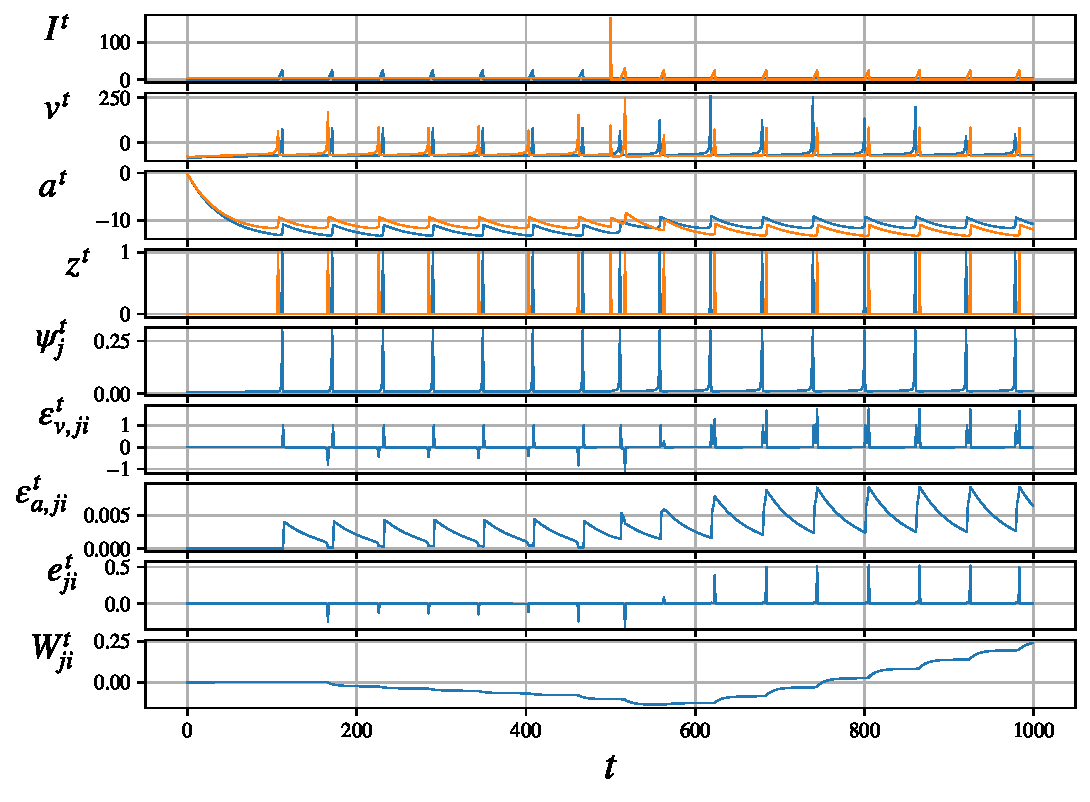
\includegraphics[width=\linewidth]{gfx/demo_izh}
    \caption{A single-synapse demo of the uncorrected Izhikevich neuron. Note that $\epsilon^t_{ji, v}$ takes on extreme values and that the eligibility vector flips sign at any pair of spikes.}
    \label{fig:demo_izh}
\end{figure}

\begin{table}[ht]
    \myfloatalign
    \begin{tabularx}{\textwidth}{lll} \toprule
        \tableheadline{Symbol} & \tableheadline{Description}
        & \tableheadline{Value} \\ \midrule
        % Phantoms take care of right-alignment (works iff monospaced digits)
        $\alpha$              & Activity leak               & 0.8 \\
        $\beta$               & Adaptivity                  & 0.184 \\
        $\rho$                & Adaptivity leak             & 0.975 \\
        $\kappa$              & Output decay                & 0.8 \\
        $\gamma$              & Pseudoderivative dampening  & 0.3 \\
        $v_\text{th}$         & Base threshold              & 0.95 \\
        $\delta t_\text{ref}$ & Refractory time             & 2 \\
        $\eta$                & Learning rate               & 0.01 \\
        $\beta_1$             & Adam momemtum factor 1      & 0.9 \\
        $\beta_2$             & Adam momemtum factor 2      & 0.999 \\
        $c_\text{reg}$        & Firing rate regularization  & 50 \\
        $c_\text{L2}$         & L2 regularization           & $10^{-5}$ \\
        $f^\text{target}$     & Target firing rate          & 0.01 \\
        $N$                   & Network size                & $800^*$ \\

		\bottomrule
    \end{tabularx}
    \caption[Hyperparameters]{The full list of hyperparameter values. \textsuperscript{*}This is the total number of neurons in multi-layer networks.}
    \label{tab:hparams}
\end{table}
